\documentclass[10pt,twocolumn,letterpaper]{article}

\usepackage{cvpr}
\usepackage{times}
\usepackage{epsfig}
\usepackage{graphicx}
\usepackage{amsmath}
\usepackage{amssymb}

% Include other packages here, before hyperref.

% If you comment hyperref and then uncomment it, you should delete
% egpaper.aux before re-running latex.  (Or just hit 'q' on the first latex
% run, let it finish, and you should be clear).
\usepackage[breaklinks=true,bookmarks=false]{hyperref}

\cvprfinalcopy % *** Uncomment this line for the final submission

\def\cvprPaperID{****} % *** Enter the CVPR Paper ID here
\def\httilde{\mbox{\tt\raisebox{-.5ex}{\symbol{126}}}}

% Pages are numbered in submission mode, and unnumbered in camera-ready
%\ifcvprfinal\pagestyle{empty}\fi
\setcounter{page}{1}
\begin{document}

%%%%%%%%% TITLE
\title{Semantic Segmentation of Urban Scenes using Fully Convolutional Networks}

\author{Zheng Luo\\
Department of Computer Science\\
University of Virginia\\
{\tt\small zl5sv@virginia.edu}
% For a paper whose authors are all at the same institution,
% omit the following lines up until the closing ``}''.
% Additional authors and addresses can be added with ``\and'',
% just like the second author.
% To save space, use either the email address or home page, not both
\and
Zixuan Lin\\
Department of Biomedical Engineering\\
University of Virginia\\
{\tt\small zl7qk@virginia.edu}
}

\maketitle
%\thispagestyle{empty}

%%%%%%%%% ABSTRACT
\begin{abstract}
   Autonomous vehicles are assumed to be the key units of the next generation transportation system. Since vehicle safety is critical to real world, it is important to maintain that a vehicle’s understanding to environment is highly reliable. Real-world driving environment is a mixture of multiple objects, and can be dense especially on urban roads. Vehicles are assumed to not only recognize multiple objects in the whole scene but also know where exactly different objects occupy. Therefore, while cameras are widely used to recognize objects, image segmentation (or clustering pixels) from a mixture becomes the challenge at the first step, in order to understand the environment precisely.
\end{abstract}




%%%%%%%%% BODY TEXT
\section{Introduction}

In this project, the plan is to cast existing different neural networks and fine tune them to segment the validation sets in Cityscapes Dataset. Finding a proper way to modify the network structures is the first important task. Moreover, we will find fine annotated training sets to train convolutional neural networks. Except playing different neural networks and compare (and try to improve) their performance of segmentation and recognition, another experiment can also be planned to test the adaptivity of trained neural networks. That is, the project is also able to study if a fine-tuned network for a single city can behave well on images from another city. Alternatively speaking, if the training set is a mixture of many different cities, it is interesting to know how much improvement can be achieved compared to only using a single or few cities.

\begin{figure}[t]
\centering
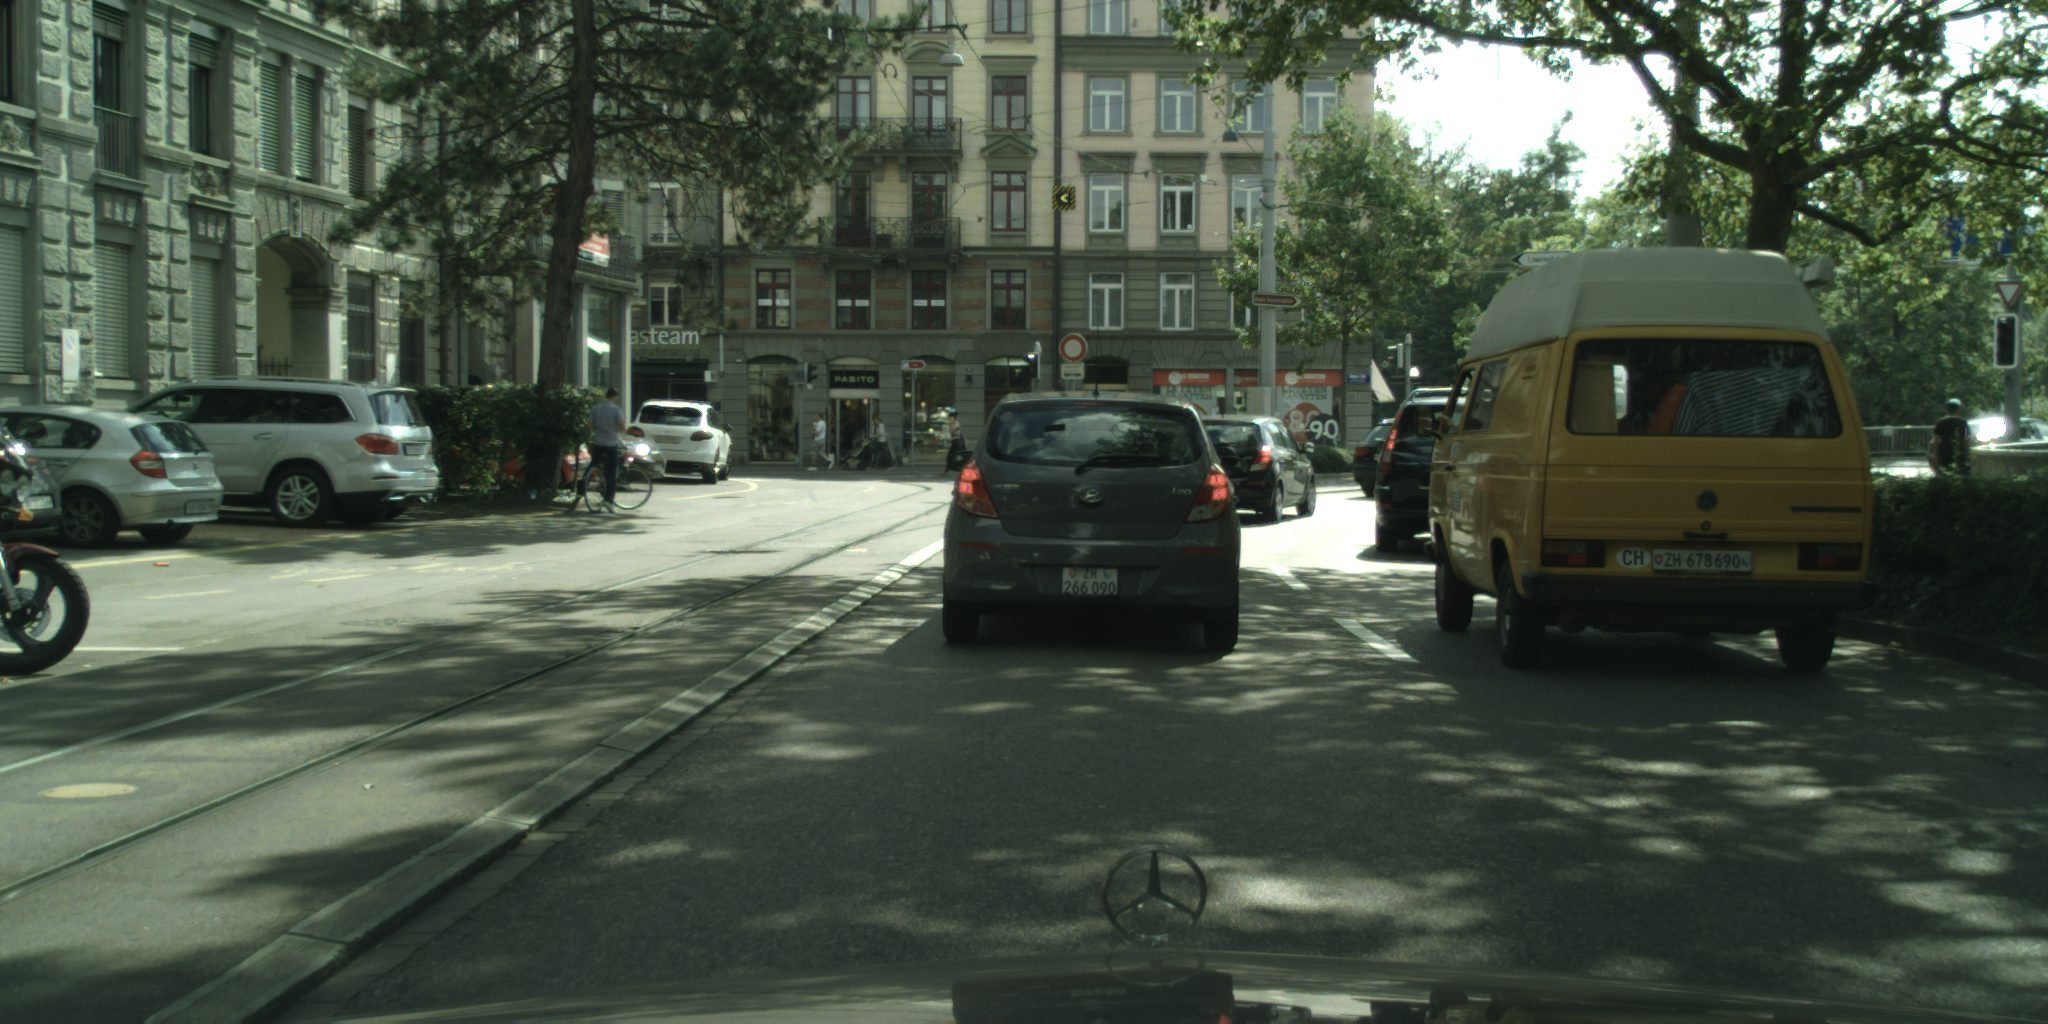
\includegraphics[width=0.40\textwidth]{zurich_example.png}
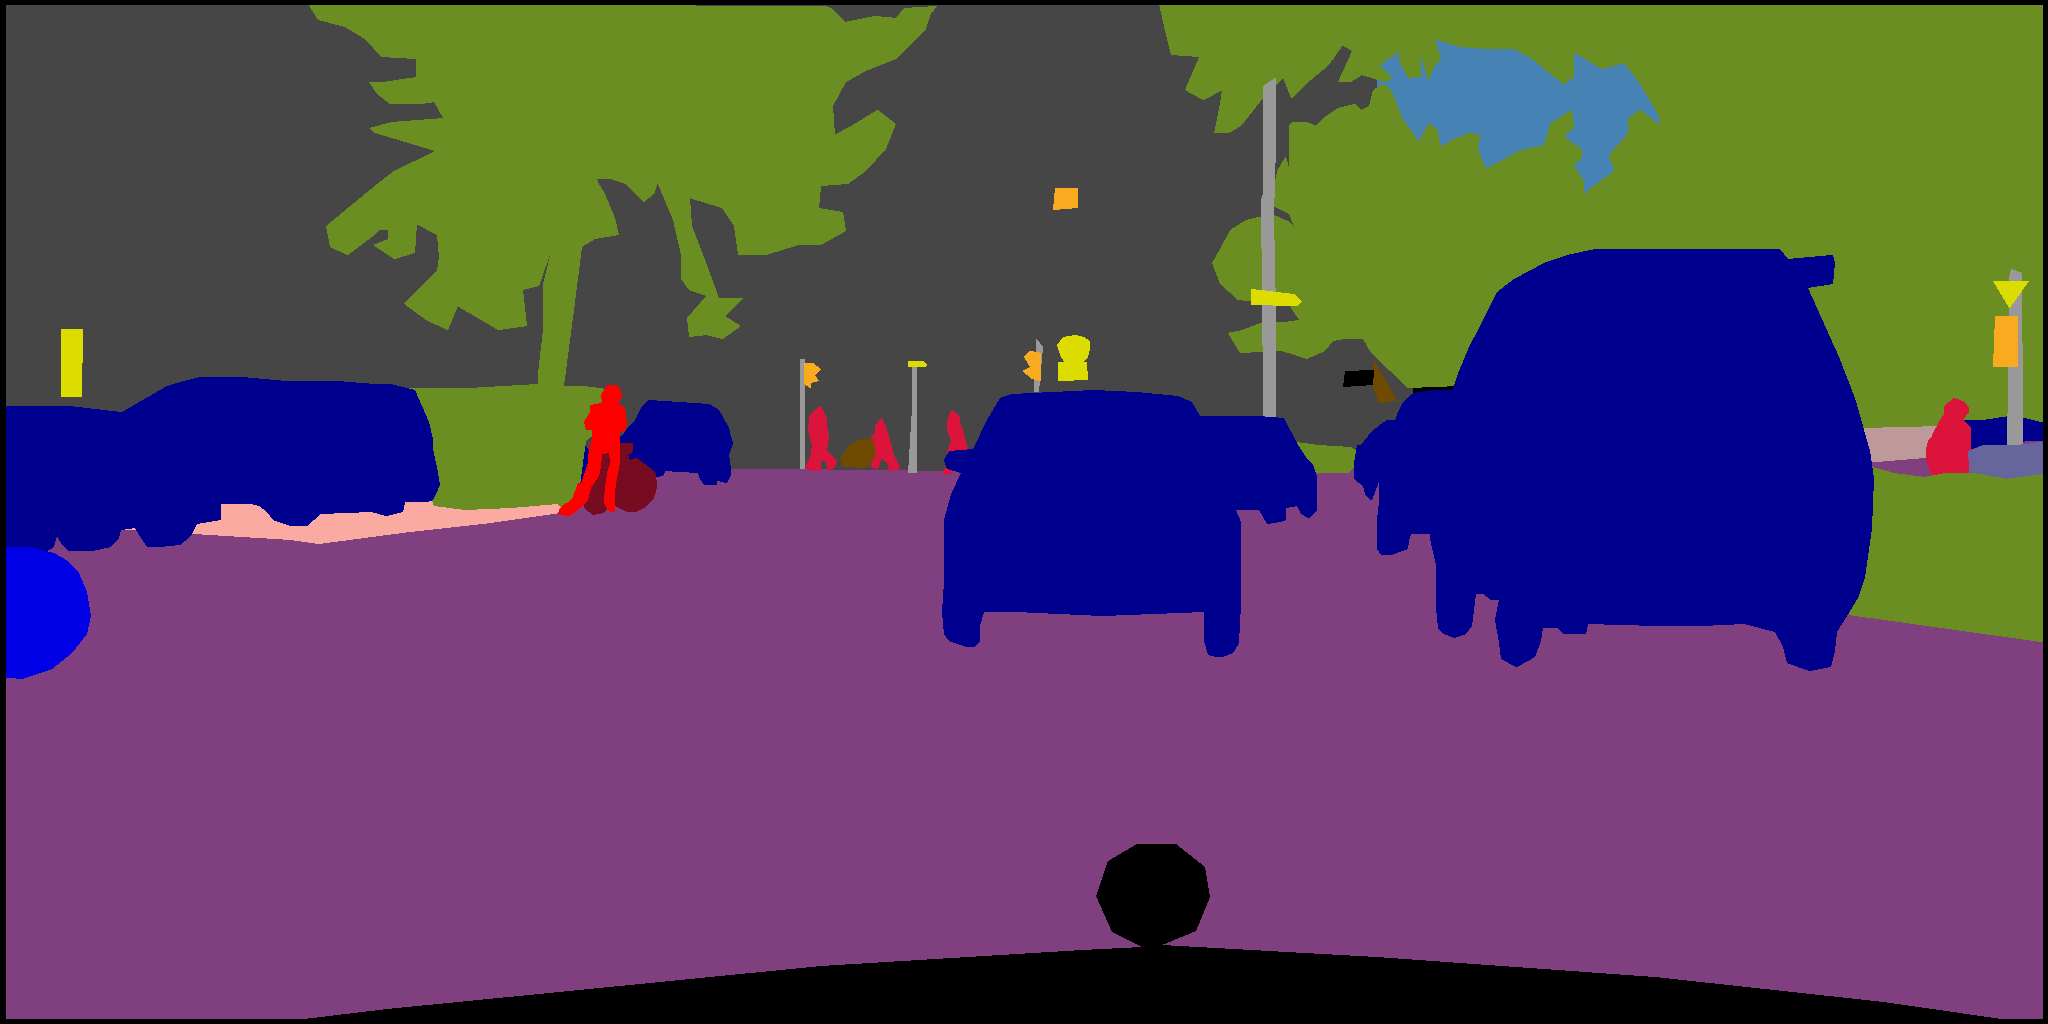
\includegraphics[width=0.40\textwidth]{zurich_example_seg.png}
\caption{Here is an illustration of fine annotated urban scene from Cityscapes Dataset. The upper side is an original image with 2048$\times$1024 resolution taken from Zuerich. The bottom side is its corresponding fine annotation. The overlayed color represents semantic classes defined by the dataset provider.}
\label{fig:leadfigure}
\end{figure}

\section{Related Work}
Proven classification architectures such as AlexNet and VGG (and their successors) are widely used for single-object recognitions. However, segmentation requires pixel-wise output to distinguish different objects rather than a single judgement. In 2015, Long et al. \cite{Long_2015_CVPR} introduced fully convolutional networks to adapt those classifiers for dense prediction, with in-network up-sampling and a pixel-wise loss. Therefore, by converting and fine tuning currently existing convolutional neural networks, it is possible to achieve a much better performance of segmentation than other simple methods such as k-means clustering and watershed transform.

Since this project is going to play a role among the problems of autonomous driving, Cityscapes Dataset \cite{Cordts2016Cityscapes} will be used in this project. It has fine annotated images and more coarse annotated images of urban scenarios from multiple cities. We will firstly use the 5000-image volumn including 3475 pixel-level fine annotated images for training and validation, and 1525 dummy annotated images for testing. The dummy annotation means regions are ignored. Class labels are defined and also grouped semantically. This dataset can be very useful due to its high quality and images resources (multiple cities). The dataset also have benchmarks for pixel-level and instance-level semantic labeling. They can be used to show segmentation performance quantitatively.


%-------------------------------------------------------------------------




{\small
\bibliographystyle{ieee}
\bibliography{egbib}
}

\end{document}
